%
% teil3.tex -- Beispiel-File für Teil 3
%
% (c) 2020 Prof Dr Andreas Müller, Hochschule Rapperswil
%
% !TEX root = ../../buch.tex
% !TEX encoding = UTF-8
%
\subsection{Mutation
\label{buch:paper:varalg:subsection:mutation}}
\rhead{Mutation}
Dieser Schritt sorgt dafür, dass zufällige Änderungen in 
den Genen stattfinden. Dadurch entstehen neue Gene, was den 
gesamten Lösungsraum vergrößert. Dies soll verhindern, 
dass nur noch gleiche Genmuster entstehen und ermöglicht 
die Erzeugung neuer Varianten. Ein guter Vergleich zum 
maschinellen Lernen ist der Versuch, aus einem lokalen 
Extrempunkt herauszukommen und nicht stecken zu bleiben.
Die Mutation findet auch nicht bei jedem Kind statt. Wie 
in der Natur können sie perzufall ausgelösst werden.
\\
Würde der genetische String nur aus 0 und 1 bestehen, 
würden zufällig Stellen ein- und ausgeschaltet. Dies 
ist mit den Städten jedoch nicht möglich, daher werden 
Teile miteinander vertauscht.

\begin{figure}
	\centering
	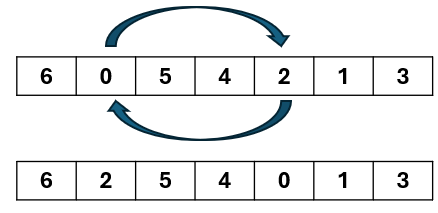
\includegraphics[width=0.8\textwidth]{
        papers/varalg/images/teil3/09GeneticStringCitiesMutation.png
        }
	\caption{Beispiel einer Mutation mit Städten}
	\label{fig:mutation_genetic_string}
\end{figure}

Dieser Teil besitzt keine mathematische Formel. Es geht einfach 
um die Logik, zwei zufällige Stellen zu nehmen und diese zu 
tauschen, um eine neue Variation von Lösungen zu erstellen, die 
bei der Kreuzung nicht entstanden wäre.
